% This is a basic version plotting from files is also available which I'll explore further
%
%
\begin{frame}{Plotting in Latex}
    Using the pgfplots package and tikz 2D and 3D plots can be made. This can also be used to plot from data files
    %
    % Define size of plots
    \pgfplotsset{width=.3 \textwidth,compat=1.9}
    % 
    \begin{figure}
        \centering
        %Here begins the 2D plot
        %
        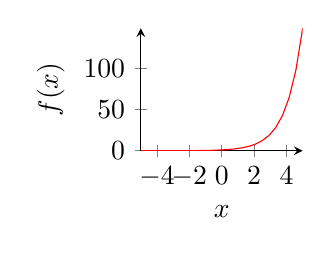
\begin{tikzpicture}
            \begin{axis}[
            axis lines = left,
            xlabel = \(x\),
            ylabel = {\(f(x)\)},
             ]
                \addplot[color=red]{exp(x)};
            \end{axis}
        \end{tikzpicture}
        % Here ends the 2D plot
        %
        \hskip .1\textwidth
        % Horizontal spacing
        %
        % Here begins the 3D plot
        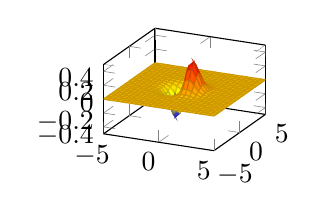
\begin{tikzpicture}
            \begin{axis}
               \addplot3[surf,]{exp(-x^2-y^2)*x};
            \end{axis}
        \end{tikzpicture}
        %Here ends the 3D plot
        \caption{Caption}
        \label{fig:fig2}
    \end{figure}

\end{frame}